\documentclass[a4paper]{article}

%\usepackage{times}
\usepackage{epsfig}
\usepackage{graphicx}
\usepackage{amsmath}
\usepackage{amsthm}
\usepackage{amssymb}
\usepackage{color}
\usepackage{subcaption}
\usepackage[left = 30mm, right = 30mm, bottom = 30mm, top = 30mm]{geometry}
\usepackage{hyperref}
\hypersetup{
	colorlinks=true,
	linkcolor=red,
	filecolor=magenta,
	urlcolor=blue,
}

% load package with ``framed'' and ``numbered'' option.
%\usepackage[framed,numbered,autolinebreaks,useliterate]{mcode}

% something NOT relevant to the usage of the package.
\setlength{\parindent}{0pt}
\setlength{\parskip}{18pt}

%\usepackage[latin1]{inputenc}
%\usepackage[T1]{fontenc}

\usepackage{listings}
\lstset{%
   language=Matlab,
   basicstyle=\small\ttfamily,
   frame=single,
}

\newcommand*\diff{\mathop{}\!\mathrm{d}}

\setlength{\fboxsep}{0pt}

\title{Pattern Recognition\\Exercise 2}
\author{Mario Kaufmann \\ Ramona Imhof \\ Jakob Sch\"arer \\ Adrian W\"alchli \\ Jan Luca Liechti}

\begin{document}

\maketitle

\section{SVM}
Using the \textit{libsvm}\footnote{\url{https://www.csie.ntu.edu.tw/~cjlin/libsvm/}} SVM library, we used the following parameters to obtain the best possible results:
\begin{itemize}
\item $k = 10$ (for k-fold cross-validation)
\item $C = 2^{-5}, \ldots, 2^{15}$ (10 different values in total)
\item $\gamma = 2^{-15}, \ldots, 2^{3}$ (10 different values in total)
\end{itemize}
With these values, we are following the \textit{libsvm} guide to support vector machines\footnote{\url{https://www.csie.ntu.edu.tw/~cjlin/papers/guide/guide.pdf}, p. 5-8.}. We also normalize all values to the interval $[0,1]$.

\section{MLP}

\subsection{Implementation with NN Toolbox}
The Neural Network toolbox from {MATLAB} was used to implement the {MLP}.
We used cross-validation to find the optimal number of neurons in the hidden layer as well as the optimal learning rate.
We adapted a grid search on the following search space:
\begin{itemize}
	\item Layer size: 50, 60, 70, ..., 150
	\item Eight learning rates on the interval $[0.001, 0.05]$
\end{itemize}
We found the optimal parameters are 140 neurons and 0.001 for the learning rate.
On the full training set, the runtime for the parameter search is about 25 minutes.
We save the performance for the best network and show it in figure~\ref{fig:perf-vs-epoch-toolbox}.
The classification accuracy on the test set with these parameters is \textbf{96.2736} percent.
\begin{figure}[tb]
	\centering
	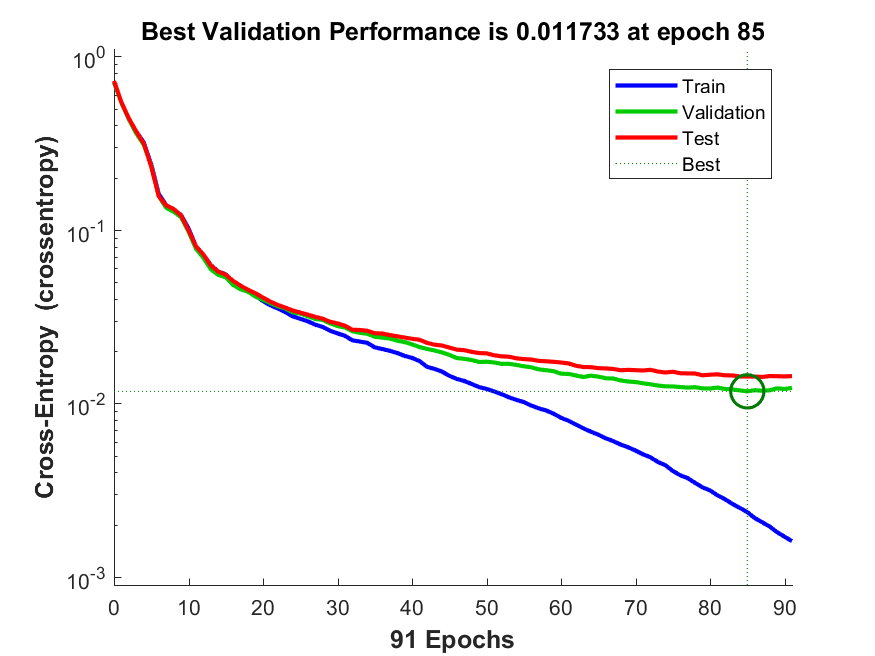
\includegraphics[width=12cm]{{images/mlp-versionB-toolbox/Performance-vs-epochs-hidden=140-LR=0.001000}.png}
	\caption{Cross-entropy error vs. epochs.
			 The test set in this figure is not the same as the test set we use for the final evaluation.
			 These are the three splits to verify the performance during training.
			 We abort after 6 validation checks (when the performance does not improve anymore).}
	\label{fig:perf-vs-epoch-toolbox}
\end{figure}

\subsection{Implementation with standard MATLAB tools}
Additionally to the solution with the neural network toolbox we implemented our own approach for training a {MLP}. It can be found in the folder \textit{mlp-regularization}. The implementation uses regularization controlled by the parameter $\lambda \in [0, 0.3]$. The other parameters were set as follows after optimization:
\begin{itemize}
	\item learning rate $c = 1$
	\item number of hidden nodes: 100
	\item number of epochs: 100
\end{itemize}
In addition, the feature descriptor \textit{HOG}\footnote{\url{http://lear.inrialpes.fr/people/triggs/pubs/Dalal-cvpr05.pdf}} was used to transform the samples into another feature space.\\
The parameter $\lambda$ heavily influences the classification accuracy. As can be seen in figure \ref{fig:results-own}, the optimal value for $\lambda$ lies around 0.1. Furthermore, it is visible that as expected, the cost is lower on the training set than on the test and validation set, just as the accuracy is lower on the test and validation set than on the training set. Under this configuration the classification accuracy was found to be \textbf{96.5936} percent on the test set.

\begin{figure}[tb]
	\centering
	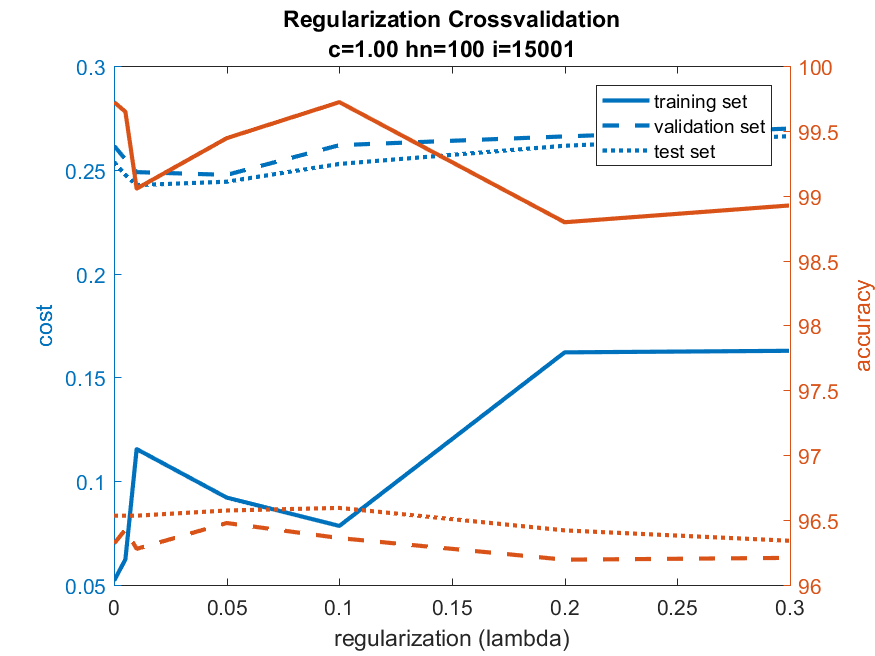
\includegraphics[width=12cm]{{images/mlp-versionA/results}.png}
	\caption{Accuracy and cost on the training, validation and test set depending on the parameter $\lambda$. The optimal value for $\lambda$ lies around 0.1.}
	\label{fig:results-own}
\end{figure}

\end{document}
